\chapter{Câu hỏi ôn tập}
\hideall{
	\setcounter{section}{0}
	\begin{center}
		\textbf{\large BẢNG ĐÁP ÁN}
	\end{center}
	\section{Câu trắc nghiệm nhiều phương án lựa chọn}
	\inputansbox{10}{ans/Y24-VN12-PH-C1-TN}
	\section{Câu trắc nghiệm đúng sai}
	\inputansbox[2]{2}{ans/Y24-VN12-PH-C1-TF}
	\section{Câu trắc nghiệm trả lời ngắn}
	\inputansbox[3]{6}{ans/Y24-VN12-PH-C1-TL}
}
\setcounter{section}{0}
\section{Câu trắc nghiệm nhiều phương án lựa chọn}
\textit{Thí sinh trả lời từ câu 1 đến câu 18. Mỗi câu thí sinh chọn một phương án}
\setcounter{ex}{0}
\Opensolutionfile{ans}[ans/Y24-VN12-PH-C1-TN]
% ===================================================================
\begin{ex}
	Chất rắn vô định hình là chất rắn
	\choice
	{có cấu trúc tinh thể}
	{\True không có cấu trúc tinh thể}
	{có nhiệt độ nóng chảy xác định}
	{có thể tích thay đổi}
	\loigiai{}
\end{ex}
% ===================================================================
\begin{ex}
	Tính chất nào sau đây \textbf{không phải} là tính chất của các phân tử khí?
	\choice
	{Có vận tốc trung bình phụ thuộc vào nhiệt độ}
	{Gây áp suất lên thành bình}
	{\True Chuyển động xung quanh vị trí cân bằng}
	{Chuyển động nhiệt hỗn loạn}
	\loigiai{}
\end{ex}
% ===================================================================
\begin{ex}
	Sự bay hơi
	\choice
	{\True xảy ra ở bất kì nhiệt độ nào của chất lỏng}
	{chỉ xảy ra ở trong lòng chất lỏng}
	{xảy ra với tốc độ như nhau ở mọi nhiệt độ}
	{chỉ xảy ra đối với một số ít chất lỏng}
	\loigiai{}
\end{ex}
% ===================================================================
\begin{ex}
	Đơn vị của nhiệt dung riêng là
		\choice
	{$\si{\joule/\kilogram}$}
	{$\si{\kilogram/\joule}$}
	{\True $\si{\joule/\kilogram\cdot\kelvin}$}
	{$\si{\kilogram/\joule\cdot\kelvin}$}
	\loigiai{}
\end{ex}
% ===================================================================
\begin{ex}
	Phát biểu nào sau đây là \textbf{sai}?
	\choice
	{Nhiệt độ sôi của chất lỏng phụ thuộc vào áp suất khí phía trên bề mặt chất lỏng}
	{Áp suất khí càng cao thì nhiệt độ sôi của chất lỏng càng cao}
	{\True Áp suất khí càng nhỏ thì nhiệt độ sôi của chất lỏng càng cao.}
	{Ở một áp suất nhất định, mỗi chất lỏng sôi ở nhiệt độ xác định và không đổi}
	\loigiai{}
\end{ex}
% ===================================================================
\begin{ex}
Nội năng của một vật là	
	\choice
	{tổng động năng chuyển động nhiệt của các phân tử cấu tạo nên vật}
	{\True tổng động năng và thế năng của các phân tử cấu tạo nên vật}
	{tổng nhiệt năng và cơ năng mà vật nhận được trong quá trình truyền nhiệt và thực hiện công}
	{nhiệt lượng vật nhận được trong quá trình truyền nhiệt}
	\loigiai{}
\end{ex}
% ===================================================================
\begin{ex}
	Nhiệt hóa hơi riêng của một chất lỏng là nhiệt lượng cần thiết để
	\choice
	{\True làm cho một kilogram chất lỏng đó hóa hơi hoàn toàn ở nhiệt độ xác định}
	{làm cho một kilogram chất lỏng tăng thêm $\SI{1}{\celsius}$}
	{làm cho một khối lượng xác định chất lỏng đó hóa hơi hoàn toàn}
	{làm cho một kilogram hơi chuyển hoàn toàn sang thể lỏng ở nhiệt độ xác định}
	\loigiai{}
\end{ex}
% ===================================================================
\begin{ex}
	Người ta thực hiện công $\SI{40}{\joule}$ lên khối khí trong xi lanh làm cho nội năng khối khí tăng thêm $\SI{20}{\joule}$ thì khối khí
	\choice
	{\True tỏa nhiệt $\SI{20}{\joule}$}
	{nhận nhiệt $\SI{20}{\joule}$}
	{tỏa nhiệt $\SI{40}{\joule}$}
	{nhận nhiệt $\SI{40}{\joule}$}
	\loigiai{}
\end{ex}
% ===================================================================
\begin{ex}
	Không thể dùng nhiệt kế rượu để đo nhiệt độ của nước đang sôi vì
	\choice
	{rượu sôi ở nhiệt độ cao hơn $\SI{100}{\celsius}$}
	{\True rượu sôi ở nhiệt độ thấp hơn $\SI{100}{\celsius}$}
	{rượu đông đặc ở nhiệt độ cao hơn $\SI{100}{\celsius}$}
	{rượu đông đặc ở nhiệt độ thấp hơn $\SI{0}{\celsius}$}
	\loigiai{}
\end{ex}
% ===================================================================
\begin{ex}
	Nhiệt độ trung bình trong 1 căn phòng ở thang nhiệt độ Celsius là $\SI{27}{\celsius}$. Nhiệt độ này trong thang nhiệt độ Kelvin là
	\choice
	{$\SI{273}{\kelvin}$}
	{\True $\SI{300}{\kelvin}$}
	{$\SI{246}{\kelvin}$}
	{$\SI{327}{\kelvin}$}
	\loigiai{}
\end{ex}
% ===================================================================
\begin{ex}
	Người ta bỏ $\SI{100}{\gram}$ nước đá ở $\SI{0}{\celsius}$ vào $\SI{300}{\gram}$ nước có nhiệt độ $\SI{30}{\celsius}$. Cho biết nhiệt nóng chảy riêng của nước đá $\lambda=\SI{3.4e5}{\joule/\kilogram}$ và nhiệt dung riêng của nước là $c =\SI{4200}{\joule/\left(\kilogram\cdot\kelvin\right)}$. Lượng nước đá còn lại chưa tan hết là
	\choice
	{$\SI{26}{\gram}$}
	{$\SI{74}{\gram}$}
	{$\SI{35}{\gram}$}
	{\True $\SI{0}{\gram}$}
	\loigiai{
	Lượng nước đá có thể tan nếu nhận nhiệt lượng do $\SI{300}{\gram}$ nước tỏa ra khi giảm nhiệt độ từ $\SI{30}{\celsius}$ xuống $\SI{0}{\celsius}$:
	$$m=\dfrac{m_nct_0}{\lambda}\approx\SI{111.12}{\gram}.$$
	}
\end{ex}
% ===================================================================
\begin{ex}
Biết nhiệt dung riêng và nhiệt nóng chảy riêng của đồng lần lượt là $c =\SI{380}{\joule/\left(\kilogram\cdot\kelvin\right)}$; $\lambda =\SI{180}{\kilo\joule/\kilogram}$; nhiệt độ nóng chảy của đồng là $\SI{1084}{\celsius}$. Nhiệt lượng cần cung cấp để nung nóng chảy hoàn toàn 1 tấn đồng từ $\SI{25}{\celsius}$ là
	\choice
	{\True $\SI{582.42E6}{\joule}$}
	{$\SI{582.42E5}{\joule}$}
	{$\SI{582.42E4}{\joule}$}
	{$\SI{582.42E3}{\joule}$}
	\loigiai{
	$Q=mc\Delta t+m\lambda=\SI{582.42E6}{\joule}$.
	}
\end{ex}
% ===================================================================
\begin{ex}
Giả thiết rằng rượu ethylic có nhiệt hoá hơi riêng là $\SI{0.9E6}{\joule/\kilogram}$  và khối lượng riêng là $\SI{0.8}{\kilogram/\liter}$. Nhiệt lượng cần thiết để $\SI{10}{\liter}$ rượu ethylic hoá hơi hoàn toàn ở nhiệt độ sôi là	
	\choice
	{$\SI{7.2E3}{\joule}$}
	{$\SI{1.125E5}{\joule}$}
	{$\SI{7.2E6}{\joule}$}
	{$\SI{9E5}{\joule}$}
	\loigiai{
	$Q=DVL=\SI{7.2E6}{\joule}.$
	}
\end{ex}
% ===================================================================
\begin{ex}
	Đun một nồi đựng $\SI{20}{\liter}$ nước ở $\SI{20}{\celsius}$ người ta dùng một bếp điện có công suất $\SI{2.5}{\kilo\watt}$, biết hiệu suất của bếp là $\SI{80}{\percent}$, nhiệt dung riêng của nước là $\SI{4200}{\joule/\kilogram\cdot\kelvin}$. Bỏ qua nhiệt lượng bếp cung cấp cho vỏ nồi, khối lượng riêng của nước là $\SI{1}{\kilogram/\liter}$. Thời gian cần thiết để đun lượng nước đến sôi là
	\choice
	{$\SI{30}{\minute}$}
	{$\SI{45}{\minute}$}
	{$\SI{56}{\minute}$}
	{$\SI{60}{\minute}$}
	\loigiai{
	Nhiệt lượng bếp cần cung cấp để đun sôi ấm:
	$$Q=\dfrac{mc\Delta t}{H}=\dfrac{20\cdot4200\cdot20}{0,8}=\SI{8.4E6}{\joule}.$$
	Thời gian dùng bếp đun:
	$$t=\dfrac{Q}{\calP}=\SI{3360}{\second}=\SI{56}{\minute}.$$
	}
\end{ex}
% ===================================================================
\begin{ex}
	Một người đặt ra một thang nhiệt độ Y, với mốc nước đá nóng chảy là $\SI{10}{\degree Y}$ và nước sôi là $\SI{60}{\degree Y}$ (ở áp suất chuẩn). Với nhiệt độ phòng là $\SI{30}{\celsius}$ thì trong thang Y là bao nhiêu độ?
	\choice
	{\True $\SI{25}{\degree Y}$}
	{$\SI{15}{\degree Y}$}
	{$\SI{35}{\degree Y}$}
	{$\SI{40}{\degree Y}$}
	\loigiai{
	$$\dfrac{Y-Y_b}{Y_s-Y_b}=\dfrac{t-t_b}{t_s-t_b}\Leftrightarrow \dfrac{Y-10}{60-10}=\dfrac{30-0}{100-0}\Rightarrow Y=\SI{25}{\degree Y}.$$
	
	}
\end{ex}
% ===================================================================
\begin{ex}
	Trong một quá trình nung nóng đẳng áp ở áp suất $\SI{1.2E5}{\pascal}$, một chất khí tăng thể tích từ $\SI{30}{\deci\meter^3}$ đến $\SI{40}{\deci\meter^3}$ và tăng nội năng một lượng là $\SI{15}{\joule}$. Biết rằng trong quá trình đẳng áp, công của hệ được tính bằng biểu thức $A'=p\Delta V$. Nhiệt lượng cần truyền cho khối khí là
	\choice
	{$\SI{1280}{\joule}$}
	{\True $\SI{1215}{\joule}$}
	{$\SI{1200}{\joule}$}
	{$\SI{1185}{\joule}$}
	\loigiai{
	Công khối khí thực hiện:
	$$A'=p\Delta V=\SI{1200}{\joule}.$$
	Nhiệt lượng cần truyền cho khối khí:
	$$Q=\Delta U-A=\Delta U+A'=\SI{1215}{\joule}.$$
	}
\end{ex}
% ===================================================================
\begin{ex}
	Một xô có chứa $M=\SI{6.8}{\kilogram}$ hỗn hợp nước và nước đá ở trong phòng. Sự thay đổi của nhiệt độ của hỗn hợp theo thời gian được biểu diễn bằng đồ thị hình bên. Lấy gần đúng nhiệt dung riêng của nước là $\SI{4200}{\joule/\left(\kilogram\cdot\kelvin\right)}$; nhiệt nóng chảy của nước đá là $\SI{3.4E5}{\joule/\kilogram}$. Cho rằng sự hấp thụ nhiệt từ môi trường là đều. Khối lượng nước đá còn lại ở thời điểm phút thứ 25 bằng bao nhiêu?
	\begin{center}
		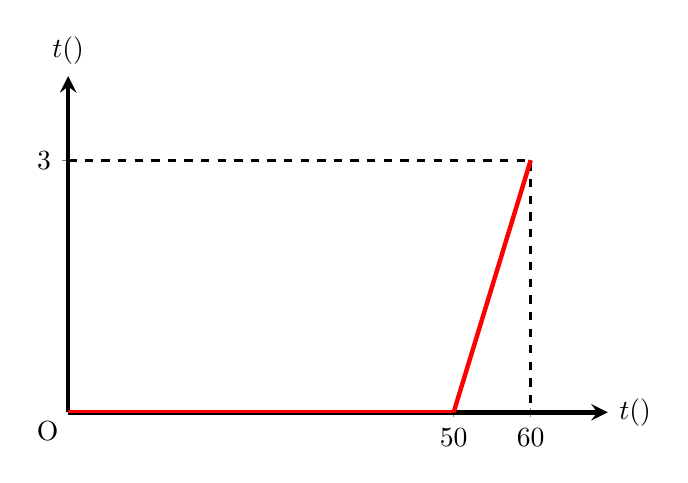
\begin{tikzpicture}  
			\begin{axis}[  ultra thick,yscale=0.75,
				xmin=0,  
				xmax=70,  
				xtick={0,50,60},
				ytick={0,3},
				ymin=0,  
				ymax=4, 
				samples=300,
				axis lines=center, 
				xlabel=$\xsi{t}{\left(\si{\minute}\right)}$, 		ylabel=$\xsi{t}{\left(\si{\celsius}\right)}$,
				every axis y label/.style={at=(current axis.above origin),anchor=south},  
				every axis x label/.style={at=(current axis.right of origin),anchor=west},  ]
				\draw[dashed, line width=1pt] (axis cs: 0,3)--++(axis cs: 60,0)--++(axis cs: 0,-3);
				\addplot [ultra thick, red, smooth, domain=0:50] {0};  
				\addplot [ultra thick, red, smooth, domain=50:60] {0.3*(x-50)} ;
				\coordinate (O) at (axis cs: 0,0) ;
				
			\end{axis}  
			\node[below left] at(O){O};
		\end{tikzpicture}
	\end{center}
	\choice
	{$\SI{5.54}{\kilogram}$}
	{\True $\SI{0.63}{\kilogram}$}
	{$\SI{0.54}{\kilogram}$}
	{$\SI{1.26}{\kilogram}$}
	\loigiai{
	Nhiệt lượng phòng tỏa ra trong khoảng thời gian từ $\SI{50}{\minute}$ đến $\SI{60}{\minute}$:
	$$Q=Mc\Delta t=\left(\SI{6.8}{\kilogram}\right)\cdot\left(\SI{4200}{\joule/\kilogram\cdot\kelvin}\right)\cdot\left(\SI{3}{\kelvin}\right)=\SI{85680}{\joule}$$
	Khối lượng nước đá trong hỗn hợp:
	$$m_{\text{đ}}=\dfrac{5Q}{\lambda}=\SI{1.26}{\kilogram}.$$
	Khối lượng nước đá còn lại ở thời điểm phút thứ 25:
	$$m'=\dfrac{m_{\text{đ}}}{2}=\SI{0.63}{\kilogram}.$$
	}
\end{ex}
% ===================================================================
\begin{ex}
	Có hai bình cách nhiệt: bình 1 chứa $\SI{2}{\kilogram}$ nước ở $\SI{20}{\celsius}$, bình 2 chứa $\SI{5}{\kilogram}$ nước ở $\SI{60}{\celsius}$. Ban đầu, người ta rót $\xsi{\Delta m}{\left(\kilogram\right)}$ nước từ bình 1 sang bình 2. Khi bình 2 cân bằng nhiệt, người ta lại rót $2\xsi{\Delta m}{\left(\kilogram\right)}$ nước từ bình 2 về bình 1. Khi bình 1 cân bằng nhiệt thì độ chênh lệch nhiệt độ giữa hai bình lúc này là $\SI{20}{\celsius}$. Giá trị của $\Delta m$ là
	\choice
	{$\SI{0.65}{\kilogram}$}
	{$\SI{0.45}{\kilogram}$}
	{\True $\SI{0.57}{\kilogram}$}
	{$\SI{0.35}{\kilogram}$}
	\loigiai{
	\textbf{* Khi rót $\Delta m$ từ bình 1 sang bình 2:}\\
	$$m_2c\left(t_{\text{cb2}}-t_2\right)+c\left(t_{\text{cb2}}-t_1\right)\Delta m=0\Rightarrow t_{\text{cb2}}=\dfrac{m_2t_2+t_1\Delta m}{m_2+\Delta m}=\dfrac{300+20\Delta m}{5+\Delta m}.$$
	\textbf{* Khi rót $2\Delta m$ từ bình 2 sang bình 1:}\\
	$$\left(m_1-\Delta m\right)c\left(t_{\text{cb1}}-t_1\right)+c\left(t_{\text{cb1}}-t_{\text{cb2}}\right)\cdot2\Delta m=0\Rightarrow t_{\text{cb1}}=\dfrac{2\left(t_{\text{cb2}}-t_{\text{cb1}}\right)\Delta m}{2-\Delta m}+20=\dfrac{40\Delta m}{2-\Delta m}+20$$
	Mà $t_{\text{cb2}}-t_{\text{cb1}}=20\Rightarrow \Delta m\approx\SI{0.57}{\kilogram}.$
	}
\end{ex}
\Closesolutionfile{ans}
\section{Câu trắc nghiệm đúng sai}
\textit{Thí sinh trả lời từ câu 1 đến câu 4. Trong mỗi ý \textbf{a)}, \textbf{b}, \textbf{c)}, \textbf{d)} ở mỗi câu, thí sinh chọn đúng hoặc sai}
\setcounter{ex}{0}
\Opensolutionfile{ans}[ans/Y24-VN12-PH-C1-TF]
% ===================================================================
\begin{ex}
	Xét cấu trúc của chất lỏng thì
	\choiceTF[t]
	{\True khoảng cách trung bình giữa các phân tử trong chất lỏng lớn hơn khoảng cách trung bình giữa các phân tử trong chất rắn và nhỏ hơn khoảng cách trung bình của các phân tử trong chất khí}
	{các phân tử chất lỏng dao động xung quanh vị trí cân bằng cố định}
	{\True chất lỏng có thể tích xác định nhưng không có hình dạng xác định mà hình dạng của nó phụ thuộc vào hình dạng của phần bình chứa nó}
	{\True lực tương tác giữa các phân tử ở thể lỏng lớn hơn lực tương tác giữa các phân tử ở thể khí}
	\loigiai{}
\end{ex}
% ===================================================================
\begin{ex}
	\immini{
		Máy thuỷ lực là một thiết bị quan trọng trong ngành xây dựng, kỹ thuật ô tô, \dots. Bên trong máy thuỷ lực người ta dùng một chất lỏng (dầu thuỷ lực). Khi ta tác dụng một lực $f$ lên piston nhỏ có diện tích $s$ lực này gây ra áp suất $p=f/s$ và được truyền nguyên vẹn đến piston lớn có diện tích $S$ và gây ra lực nâng $F$.	
	}
	{
		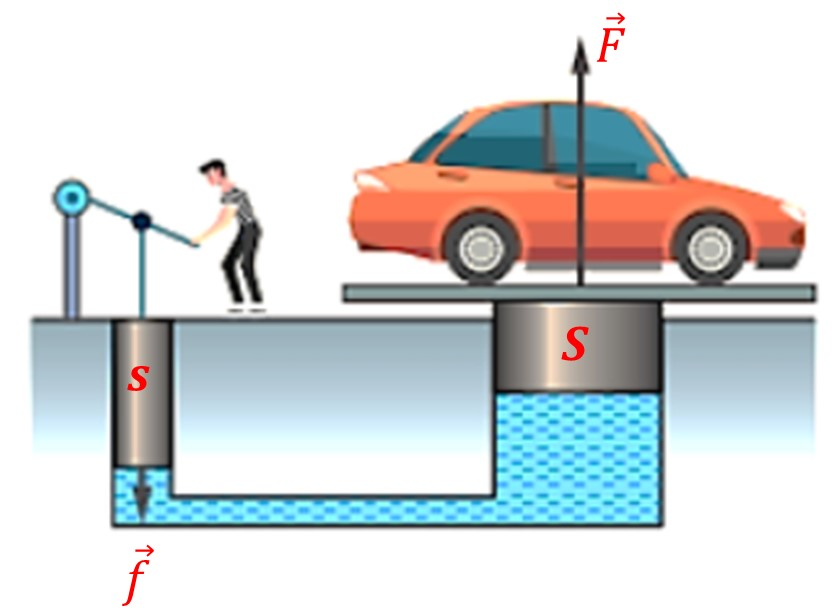
\includegraphics[width=0.6\linewidth]{../figs/Y24-VN12-PH-C1-BT-1}
	}
	\choiceTF[t]
	{Có thể thay thế chất lỏng trong máy thuỷ lực bằng chất khí}
	{Người ta sử dụng dầu thuỷ lực vì dầu thuỷ lực có đặc tính rất khó bị nén}
	{\True Nếu người ta nén với lực $f$ rất lón, các phân tử chất lỏng trong máy thuỷ lực càng bị nén chặt và có thể chuyển sang thể rắn}
	{Giả sử piston lớn có diện tích gấp 50 lần piston nhỏ. Khi đó, nếu muốn nâng một xe có khối lượng $\SI{1500}{\kilogram}$ thì cần tác dụng lên piston nhỏ một lực $\SI{30}{\newton}$}
	\loigiai{
		\begin{itemchoice}
			\itemch Sai. Vì chất khí dễ bị nén nên máy không hoạt động được.
			\itemch Đúng.
			\itemch Sai. Chất lỏng không thể chuyển thành thể rắn khi chỉ bị nén.
			\itemch Sai. $p=\dfrac{f}{s}=\dfrac{F}{S}\Rightarrow f=\dfrac{Fs}{S}=\SI{300}{\newton}$.
			
		\end{itemchoice}	
	}
\end{ex}
% ===================================================================
\begin{ex}
	Một khối băng có khối lượng $m =\SI{800}{\gram}$ ở $\SI{-10}{\celsius}$. Biết nhiệt dung riêng của nước đá là $c_{\text{đ}}= \SI{2090}{\joule/\kilogram\cdot\kelvin}$; nhiệt dung riêng của nước là $c_n =\SI{4190}{\joule/\kilogram\cdot\kelvin}$ và nhiệt nóng chảy riêng của nước đá $\lambda=\SI{3.33E5}{\joule/\kilogram}$.
	\choiceTF[t]
	{Để nóng chảy hoàn toàn, khối băng cần nhận được một năng lượng xấp xỉ $\SI{16720}{\joule}$}
	{Khi ở  $\SI{0}{\celsius}$, nếu truyền một nhiệt lượng $\SI{3352}{\joule}$ thì khối băng tan hoàn toàn thành nước ở nhiệt độ $\SI{0}{\celsius}$}
	{\True Khi băng bắt đầu nóng chảy, nếu nhận được nhiệt lượng $\SI{83.25}{\kilo\joule}$ thì khối lượng băng còn lại là $\SI{550}{\gram}$}
	{\True Cần một năng lượng $\SI{336.92}{\kilo\joule}$ truyền cho khối băng để nó chuyển hoàn toàn sang trạng thái lỏng ở $\SI{25}{\celsius}$}
	\loigiai{
	\begin{itemchoice}
		\itemch Sai. $Q=mc_{\text{đ}}\Delta t+m\lambda=\SI{283120}{\joule}$.
		\itemch Sai. $Q=m\lambda=\SI{266400}{\joule}$.
		\itemch Đúng.
		\itemch Đúng.
	\end{itemchoice}
	}
\end{ex}
% ===================================================================
\begin{ex}
	Người ta dùng một lò hồ quang điện để nấu chảy một khối kim loại nặng $\SI{29}{\kilogram}$. Biết mỗi phút lò hồ quang cung cấp cho khối kim loại một nhiệt lượng không đổi là $\SI{400}{\kilo\joule}$. Sự thay đổi nhiệt độ của khối kim loại được ghi lại theo thời gian như hình vẽ.
	\begin{center}
		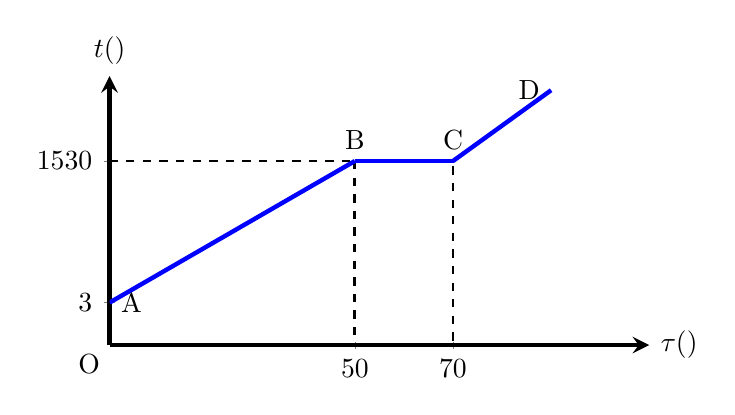
\begin{tikzpicture}  
			\begin{axis}[  ultra thick,yscale=0.6,
				xmin=0,  
				xmax=110,  
				xtick={0,50,70},
				ytick={0,3,13},
				yticklabels={0,3,1530},
				ymin=0,  
				ymax=19, 
				samples=300,
				axis lines=center, 
				xlabel=$\xsi{\tau}{\left(\si{\minute}\right)}$, 		ylabel=$\xsi{t}{\left(\si{\celsius}\right)}$,
				every axis y label/.style={at=(current axis.above origin),anchor=south},  
				every axis x label/.style={at=(current axis.right of origin),anchor=west},  ]
				\draw[dashed, line width=1pt] (axis cs: 0,13)--++(axis cs: 70,0)--++(axis cs: 0,-13);
				\draw[dashed, line width=1pt] (axis cs: 50,13)--(axis cs: 50,0);
				\addplot [ultra thick, blue, smooth, domain=0:50] {3+0.2*x};  
				\addplot [ultra thick, blue, smooth, domain=50:70] {13};
				\addplot [ultra thick, blue, smooth, domain=70:90] {13+0.25*(x-70)};
				\node[right] at (0,3) {A};
				\node[above] at (50,13) {B};
				\node[above] at (70,13) {C};
				\node[left] at (90,18) {D};
				\coordinate (O) at (axis cs: 0,0);
			\end{axis}  
			\node[below left] at (O) {O};
		\end{tikzpicture}
	\end{center}
	\choiceTF[t]
	{Giai đoạn AB trên đồ thị tương ứng với quá trình nóng chảy của kim loại}
	{Giai đoạn BC khối kim loại không nhận thêm nhiệt lượng từ lò nung}
	{\True Nhiệt dung riêng của khối kim loại xấp xỉ $\SI{459.8}{\joule/\kilogram\cdot\kelvin}$}
	{\True Nhiệt nóng chảy riêng của khối kim loại xấp xỉ $\SI{276E3}{\joule/\kilogram}$}
	\loigiai{
	\begin{itemchoice}
		\itemch Sai. Giai đoạn AB khối kim loại được nung nóng và đang tăng nhiệt độ.
		\itemch Sai. Khối kim loại vẫn nhận thêm nhiệt lượng và đang nóng chảy.
		\itemch Đúng.
		\itemch Đúng.
	\end{itemchoice}
	}
\end{ex}
\Closesolutionfile{ans}
\section{Câu trắc nghiệm trả lời ngắn} \textit{Thí sinh trả lời từ câu 1 đến câu 6}
\setcounter{ex}{0}
\Opensolutionfile{ans}[ans/Y24-VN12-PH-C1-TL]
% ===============================================================
\begin{ex}
Những viên nước đá ở $\SI{0}{\celsius}$ và khối lượng mỗi viên là $\SI{200}{\gram}$ lần lượt được thả vào $\SI{2}{\kilogram}$ nước ở $\SI{32}{\celsius}$ sao cho khi viên nước đá trước khi tan hết thì viên tiếp theo mới được thả vào. Cho biết năng lượng nhiệt cần thiết để làm tan $\SI{1}{\gram}$ nước đá  là $\SI{334}{\joule}$ và nhiệt dung riêng của nước là $\SI{4.18}{\joule/\left(\gram\cdot\kelvin\right)}$. Xác định số viên đá tối đa có thể thả vào lượng nước trên để trong nước không còn sót lại phần đá nào.	
	\shortans{4}
	\loigiai{
		Nhiệt lượng nước tỏa ra để giảm từ $\SI{32}{\celsius}$ xuống còn $\SI{0}{\celsius}$ có thể làm tan tối đa số viên đá là:
		$$N=\dfrac{m_nct_0}{\lambda m_\text{đ}}=4,005.$$
	}
\end{ex}
% ===============================================================
\begin{ex}
Biết rằng khoảng cách mỗi độ chia trong thang đo nhiệt độ X tương ứng với 1,5 độ chia trong thang đo nhiệt độ Y. Một vật khi có nhiệt độ $\SI{25}{\degree X}$ sẽ có nhiệt độ tương ứng là $\SI{45}{\degree Y}$ trong thang đo nhiệt độ Y. Khi nhiệt độ đo được ở thang Y là $\SI{50}{\degree Y}$ thì nhiệt độ tương ứng trong thang X là bao nhiêu $\si{\degree X}$?	
	\shortans{32,5 }
	\loigiai{
		$$\left(T_X-\SI{25}{\degree X}\right)\cdot1=\left(T_Y-\SI{45}{\degree Y}\right)\cdot 1,5\Rightarrow T_X=1,5T_Y-42,5$$
		Khi $T_Y=\SI{50}{\degree Y}$ thì $T_X=\SI{32.5}{\degree X}$.
	}
\end{ex}
% ===============================================================
\begin{ex}
Một khối khí được đặt trong một xilanh nằm ngang, được đậy kín bằng một pit-tông. Người ta cung cấp cho khối khí một nhiệt lượng $\SI{5}{\joule}$. Lúc này khối khí nở ra và đẩy pit-tông dịch chuyển (coi là chuyển động đều) một đoạn $\SI{10}{\centi\meter}$. Biết rằng lực ma sát giữa pit-tông và xilanh có độ lớn $F_{\text{ms}} =\SI{10}{\newton}$. Tính độ biến thiên nội năng của khối khí theo đơn vị $\si{\joule}$.	
	\shortans{4}
	\loigiai{
	Công do khối khí thực hiện:
	$$A'=Fs=\left(\SI{10}{\newton}\right)\cdot\left(\SI{0.1}{\meter}\right)=\SI{1}{\joule}.$$
	Độ biến thiên nội năng của khối khí:
	$$\Delta U=Q+A=Q-A'=\SI{4}{\joule}.$$	
	}
\end{ex}
% ===============================================================
\begin{ex}
	Một người cọ xát một miếng sắt dẹt có khối lượng $\SI{150}{\gram}$ trên một tấm đá mài. Sau một khoảng thời gian, miếng sắt nóng thêm $\SI{12}{\celsius}$. Giả sử rằng $\SI{40}{\percent}$ công đó được dùng để làm nóng miếng sắt. Biết nhiệt dung riêng của sắt là $\SI{460}{\joule/\kilogram\cdot\kelvin}$. Công mà người này đã thực hiện là bao nhiêu $\si{\joule}$?
	\shortans{2070 }
	\loigiai{
		$A=\dfrac{mc\Delta t}{H}=\SI{2070}{\joule}.$
	}
\end{ex}
% ===============================================================
\begin{ex}
Trong thí nghiệm đo nhiệt dung riêng của nước, công suất điện trên oát kế là $\SI{950}{\watt}$, khối lượng nước được sử dụng là $\SI{1}{\kilogram}$. Đồ thị thực nghiệm nhiệt độ phụ thuộc vào thời gian xác định được như hình bên dưới.
\begin{center}
	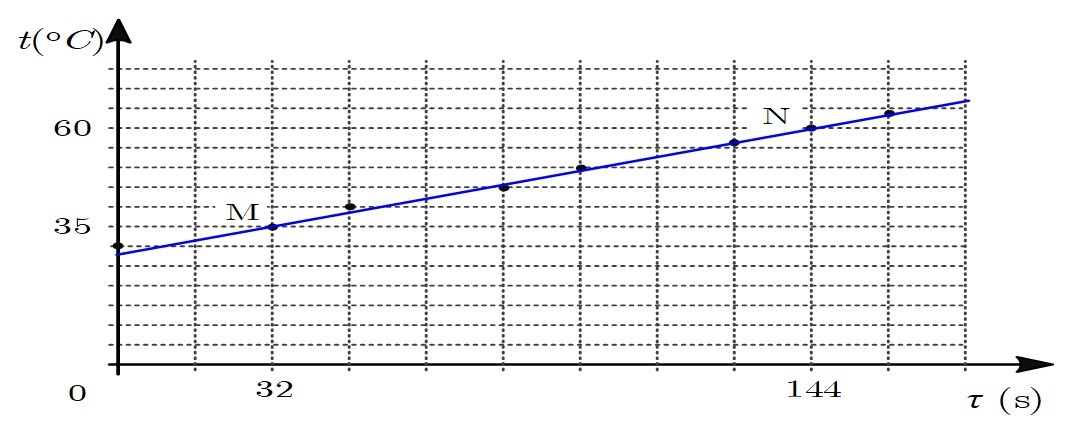
\includegraphics[width=0.7\linewidth]{../figs/Y24-VN12-PH-C1-BT-2}
\end{center}	
Hãy tính nhiệt dung riêng của nước ra đơn vị J/kg.K.
	\shortans{ 4256}
	\loigiai{
		$$c=\dfrac{\calP t}{m\Delta t}=\dfrac{\left(\SI{950}{\watt}\right)\cdot\left(\SI{144}{\second}-\SI{32}{\second}\right)}{\left(\SI{1}{\kilogram}\right)\cdot\left(\SI{60}{\celsius}-\SI{35}{\celsius}\right)}=\SI{4256}{\joule/\kilogram\cdot\kelvin}.$$
	}
\end{ex}
% ===============================================================
\begin{ex}
Có ba bình nước giống nhau, mỗi bình chứa $\SI{20}{\gram}$ nước ở cùng nhiệt độ. Người ta thả vào mỗi bình một cục nước đá có khối lượng khác nhau nhưng có cùng nhiệt độ. Bình 1 được thả cục nước đá có khối lượng $\SI{10}{\gram}$, khi cân bằng nhiệt, khối lượng nước đá còn lại trong bình là $\SI{9}{\gram}$. Bình 2 được thả cục nước đá có khối lượng $\SI{20}{\gram}$, khi cân bằng nhiệt, khối lượng nước đá trong bình không đổi. Bình 3 được thả cục nước đá có khối lượng $\SI{40}{\gram}$, khi có cân bằng nhiệt, khối lượng nước đá trong bình là bao nhiêu gram?	
	\shortans{42 }
	\loigiai{
		Bình 1 chỉ có $\Delta m_1=\SI{1}{\gram}$ đá tan thành nước $\Rightarrow$ nhiệt độ cân bằng của hỗn hợp là $\SI{0}{\celsius}$:
		$$m_nc_nt_n=m_{\text{đ1}}c\left(0-t_{\text{đ}}\right)+\lambda\Delta m_1$$
		\begin{equation}
			\Rightarrow 20c_nt_n=-10ct_{\text{đ}}+\lambda
			\label{eq: 1}
		\end{equation}
		Bình 2 có khối lượng nước đá không đổi, chứng tỏ nhiệt lượng nước tỏa ra để giảm nhiệt độ xuống $\SI{0}{\celsius}$ bằng nhiệt lượng nước đá thu vào để tăng nhiệt độ lên $\SI{0}{\celsius}$.
		\begin{equation}
			m_nc_nt_n=-m_{\text{đ2}}ct_{\text{đ}}
			\Leftrightarrow c_nt_n=-c_\text{đ}t_{\text{đ}}
			\label{eq: 2}
		\end{equation}
		Từ \eqref{eq: 1} và \eqref{eq: 2}, suy ra:
		$$\begin{cases}
		c_nt_n=0,1\lambda\\
			ct_{\text{đ}}=-0,1\lambda
		\end{cases}$$
		Bình 3 được thả cục nước đá có khối lượng $\SI{40}{\gram}$ nên nước sẽ bị đóng băng, khối lượng nước đóng băng là $m_{\text{b}}$:
		$$m_nc_nt_n+m_b\lambda=-m_{\text{đ3}}ct_{\text{đ}}\Leftrightarrow 20\cdot0,1\lambda+m_b\lambda=40\cdot0,1\lambda\Rightarrow m_{\text{b}}=\SI{2}{\gram}.$$
		Vậy bình 3 khi cân bằng nhiệt thì khối lượng nước đá là $m_{\text{đ3}}+m_{\text{b}}=\SI{42}{\gram}.$
	}
\end{ex}
\Closesolutionfile{ans}

